\documentclass[12pt,titlepage]{article}
\usepackage[margin=1.25in]{geometry}
\usepackage{graphicx,amsmath,blindtext,minted}

%% Variables definition
\newcommand{\vSubject}{Advanced Web Programming}
\newcommand{\vSubtitle}{Routing, Controller, Dan View}
\newcommand{\vName}{Muhammad Baihaqi Aulia Asy'ari}
\newcommand{\vNIM}{2241720145}
\newcommand{\vClass}{2I}
\newcommand{\vDepartment}{Information Technology}
\newcommand{\vStudyProgram}{D4 Informatics Engineering}

%% [START] Tikz related stuff
\usepackage{tikz}
\usetikzlibrary{svg.path,calc,shapes.geometric,shapes.misc}
\tikzstyle{terminator} = [rectangle, draw, text centered, rounded corners = 1em, minimum height=2em]
\tikzstyle{preparation} = [chamfered rectangle, chamfered rectangle sep=0.75em, draw, text centered, minimum height = 2em]
\tikzstyle{process} = [rectangle, draw, text centered, minimum height=2em]
\tikzstyle{decision} = [diamond, aspect=2, draw, text centered, minimum height=2em]
\tikzstyle{data}=[trapezium, draw, text centered, trapezium left angle=60, trapezium right angle=120, minimum height=2em]
\tikzstyle{connector} = [line width=0.25mm,->]
%% [END] Tikz related stuff

%% [START] Fancy header related stuff
\usepackage{fancyhdr}
\pagestyle{fancy}
\setlength{\headheight}{15pt} % compensate fancyhdr style
\fancyhead{}
\fancyfoot{}
\fancyfoot[L]{\thepage}
\fancyfoot[R]{\textit{\vSubject - \vSubtitle}}
\renewcommand{\footrulewidth}{0.4pt}% default is 0pt, overline for footer
%% [END] Fancy header related stuff

%% [START] Custom tabular command related stuff
\usepackage{tabularx}
\newcommand{\details}[2]{
    #1 & #2  \\
}
%% [END] Custom tabular command related stuff

%% [START] Figure related stuff
\newcommand{\image}[3][1]{
    \begin{figure}[h]
        \centering
        \includegraphics[#1]{#2}
        \caption{#3}
        \label{#3}
    \end{figure}
}
%% [END] Figure related stuff

%%
\usepackage{pgf-umlcd}

\renewcommand{\umldrawcolor}{black}
\renewcommand{\umlfillcolor}{white}
%%

%% [BEGIN] Custom enumerator
\usepackage{enumitem}
%% [END] Custom enumerator

%% [BEGIN] Paragraph indent
\usepackage{indentfirst}
%% [END] Paragraph indent

%% [BEGIN] URL
\usepackage{hyperref}
\hypersetup{
    colorlinks=true,
    linkcolor=blue,
    filecolor=magenta,      
    urlcolor=cyan,
    pdftitle={Overleaf Example},
    pdfpagemode=FullScreen,
    }

\urlstyle{same}
%% [END] URL

\begin{document}
\begin{titlepage}
    \centering
    \vfill
    {\bfseries\LARGE
        \vSubject\\
        \vskip0.25cm
        \vSubtitle
    }
    \vfill
    
\includegraphics[width=6cm]{images/polinema-logo.png}
    \vfill
    {
        \textbf{Name}\\
        \vName\\
        \vskip0.5cm
        \textbf{NIM}\\
        \vNIM\\
        \vskip0.5cm
        \textbf{Class}\\
        \vClass\\
        \vskip0.5cm
        \textbf{Department}\\
        \vDepartment\\
        \vskip0.5cm
        \textbf{Study Program}\\
        \vStudyProgram
    }
\end{titlepage}

\newpage

\section{Routing}
\subsection{Basic Routing}

\begin{enumerate}[label=\alph*.]
    \item -
    \item -
    \begin{minted}[autogobble,breaklines,linenos]{php}
        <?php

        use Illuminate\Support\Facades\Route;
        
        /*
        |--------------------------------------------------------------------------
        | Web Routes
        |--------------------------------------------------------------------------
        |
        | Here is where you can register web routes for your application. These
        | routes are loaded by the RouteServiceProvider and all of them will
        | be assigned to the "web" middleware group. Make something great!
        |
        */
        
        Route::get('/', function () {
            return view('welcome');
        });
        
        Route::get('/hello', function () {
            return 'Hello World';
        });
    \end{minted}
    \newpage
    \item - \\ 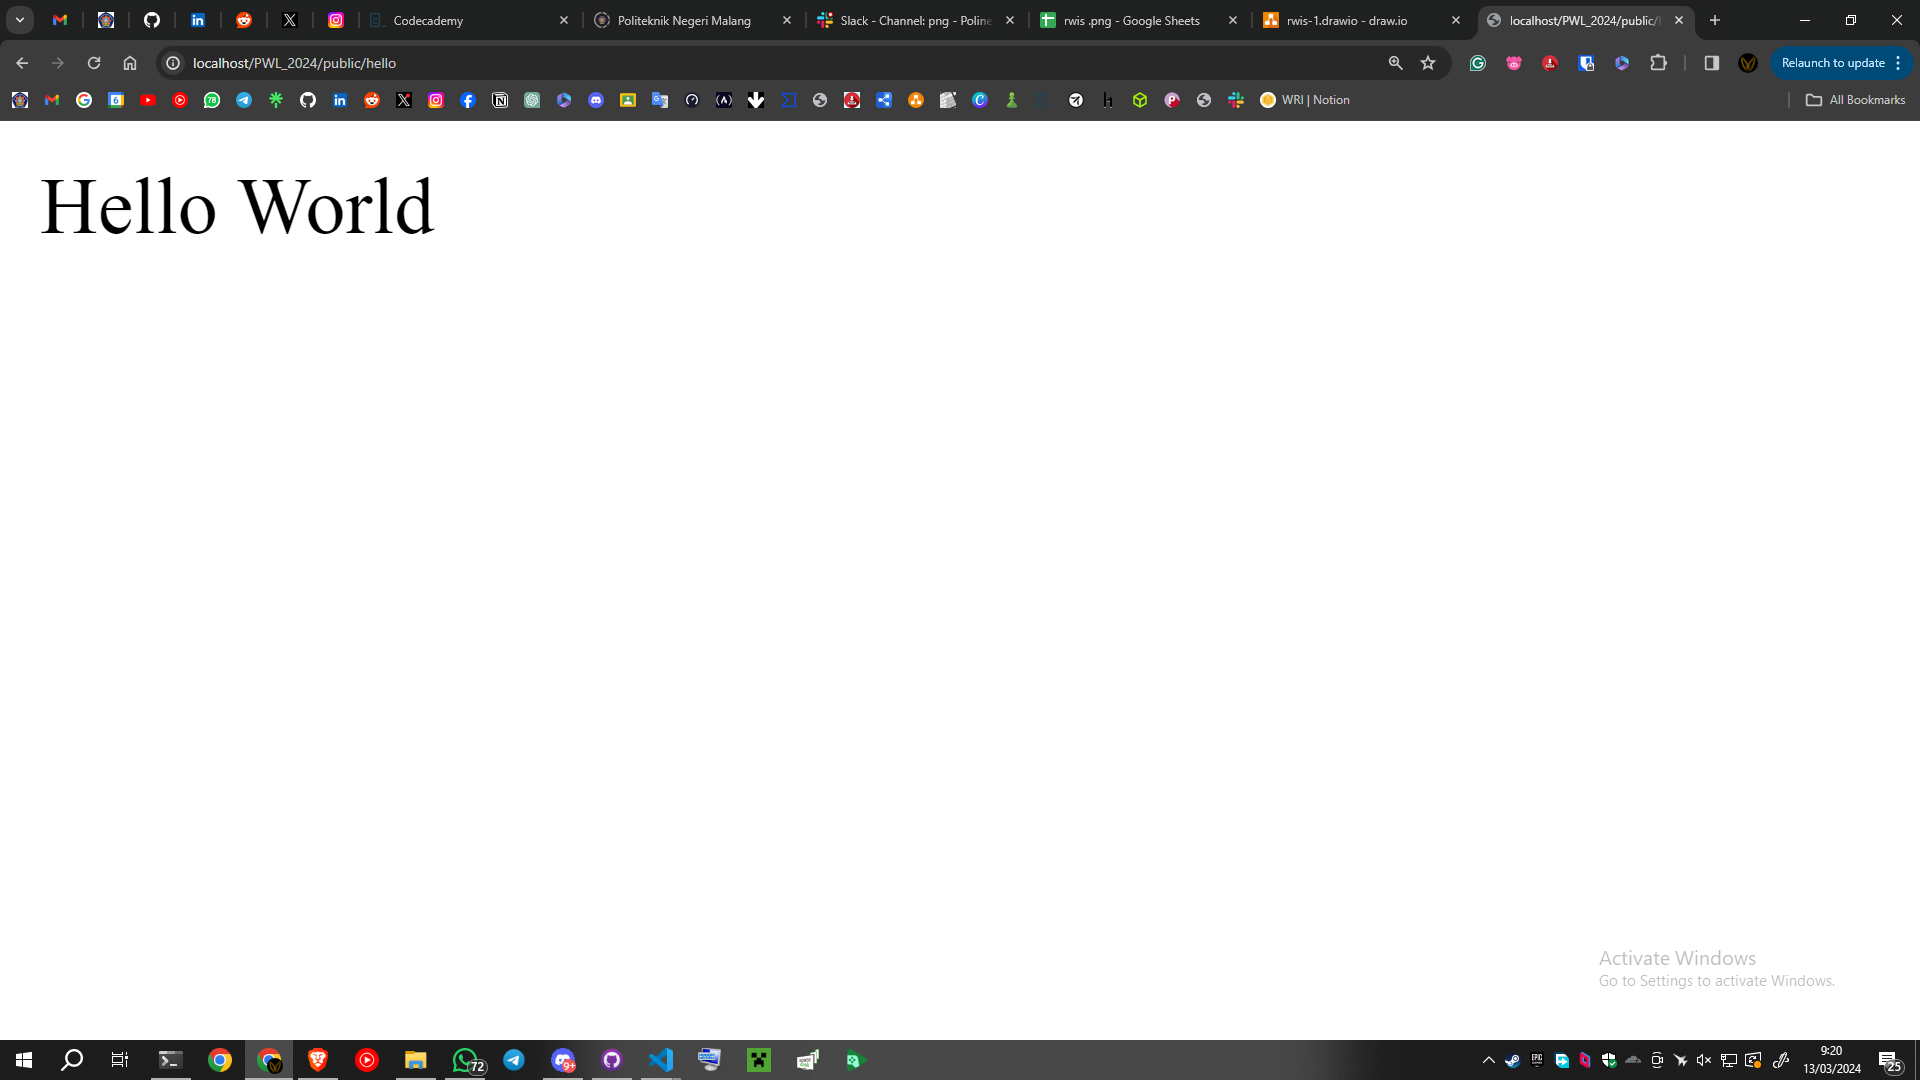
\includegraphics[width=.9\textwidth]{images/figures/basic routing c.png} \\ a 'Hello World' text appear on the page
    \newpage
    \item -
    \begin{minted}[autogobble,breaklines,linenos]{php}
        <?php

        use Illuminate\Support\Facades\Route;
        
        /*
        |--------------------------------------------------------------------------
        | Web Routes
        |--------------------------------------------------------------------------
        |
        | Here is where you can register web routes for your application. These
        | routes are loaded by the RouteServiceProvider and all of them will
        | be assigned to the "web" middleware group. Make something great!
        |
        */
        
        Route::get('/', function () {
            return view('welcome');
        });
        
        Route::get('/hello', function () {
            return 'Hello World';
        });
        
        Route::get('/world', function () {
            return 'World';
        }); 
    \end{minted}
    \newpage
    \item -\\ 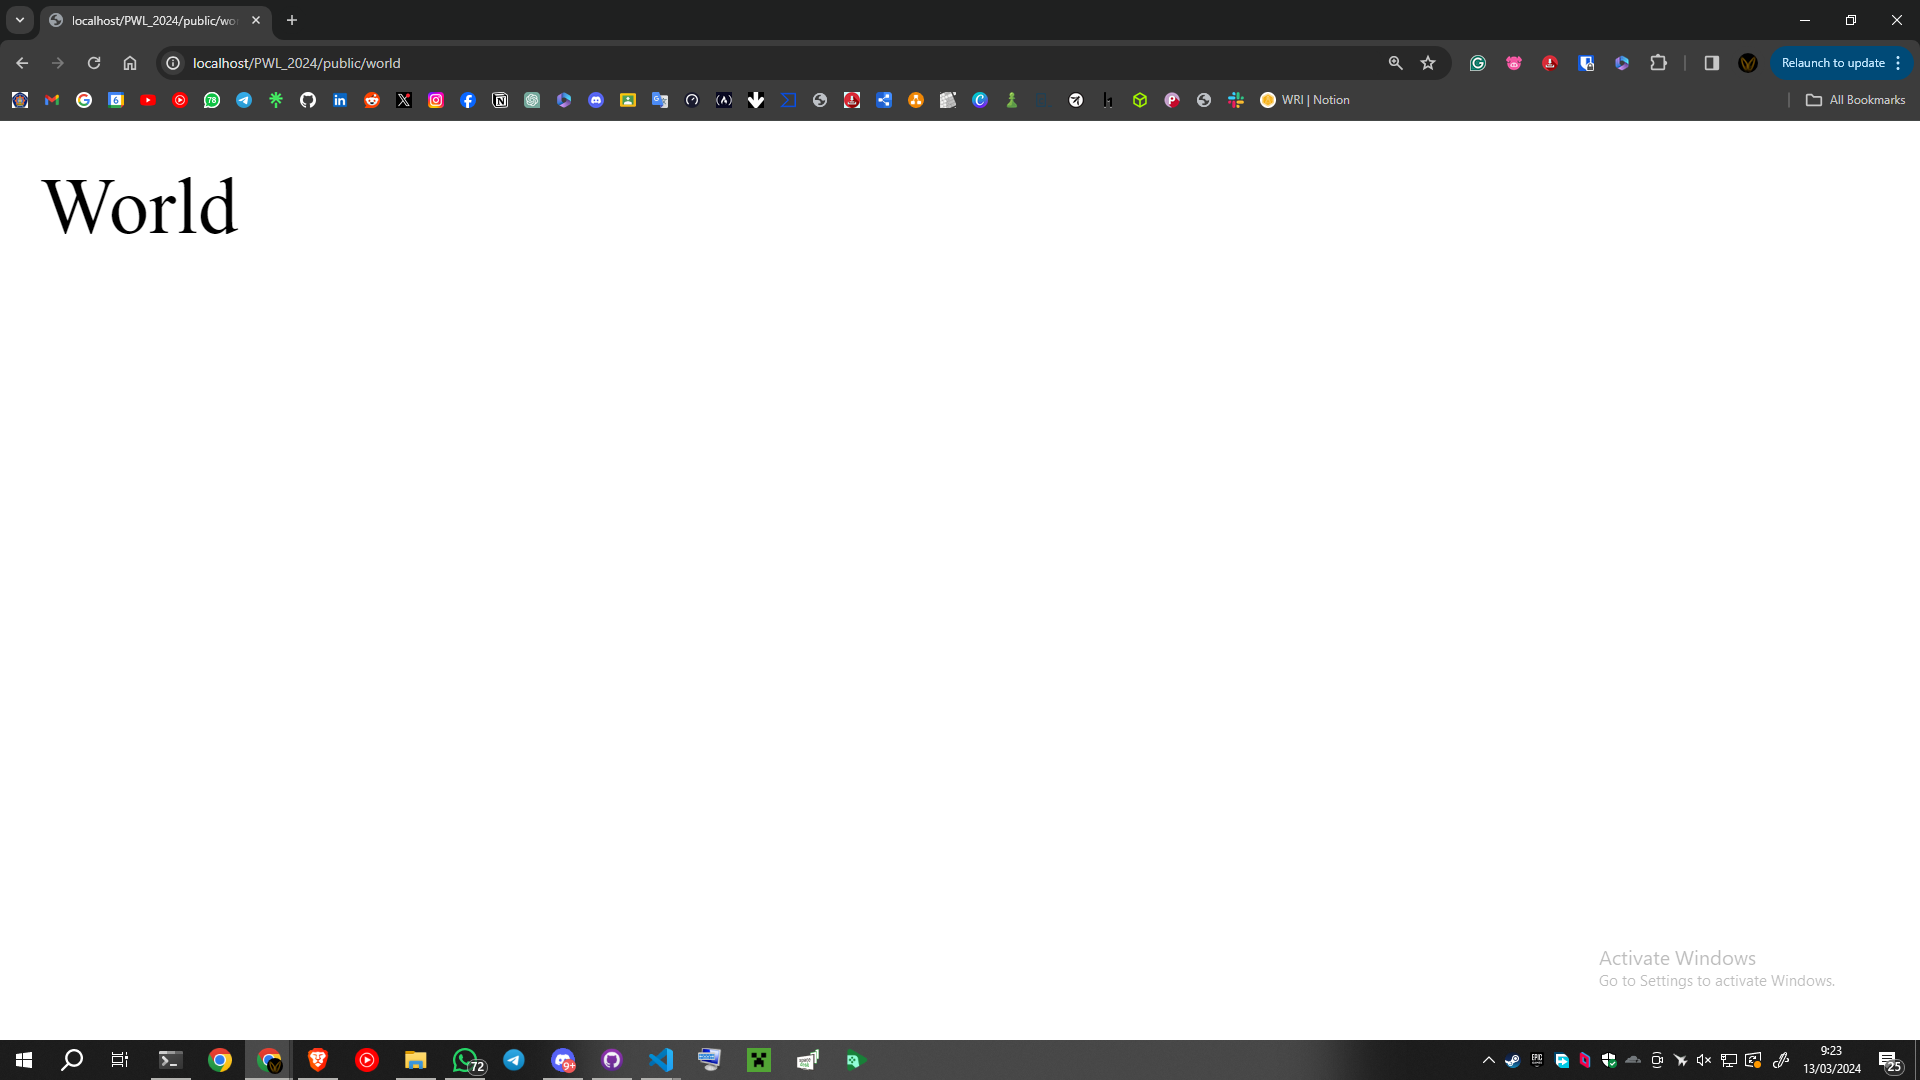
\includegraphics[width=.9\textwidth]{images/figures/basic routing e.png} \\ only the word 'World' appear on the page
    \item - \\ \includegraphics[width=.9\textwidth]{images/figures/basic routing f.png}
    \begin{minted}[autogobble,breaklines,linenos]{php}
        <?php

        use Illuminate\Support\Facades\Route;
        
        /*
        |--------------------------------------------------------------------------
        | Web Routes
        |--------------------------------------------------------------------------
        |
        | Here is where you can register web routes for your application. These
        | routes are loaded by the RouteServiceProvider and all of them will
        | be assigned to the "web" middleware group. Make something great!
        |
        */
        
        Route::get('/', function () {
            // return view('welcome');
            return 'Welcome';
        });
        
        Route::get('/hello', function () {
            return 'Hello World';
        });
        
        Route::get('/world', function () {
            return 'World';
        });
    \end{minted}
    \item - \\ \includegraphics[width=.9\textwidth]{images/figures/basic routing g.png}
    \begin{minted}[autogobble,breaklines,linenos]{php}
        <?php

        use Illuminate\Support\Facades\Route;
        
        /*
        |--------------------------------------------------------------------------
        | Web Routes
        |--------------------------------------------------------------------------
        |
        | Here is where you can register web routes for your application. These
        | routes are loaded by the RouteServiceProvider and all of them will
        | be assigned to the "web" middleware group. Make something great!
        |
        */
        
        Route::get('/', function () {
            // return view('welcome');
            return 'Welcome';
        });
        
        Route::get('/hello', function () {
            return 'Hello World';
        });
        
        Route::get('/world', function () {
            return 'World';
        }); 
        
        Route::get('/about', function () {
            return '2241720145 - Muhammad Baihaqi Aulia Asyari';
        });
    \end{minted}
\end{enumerate}

\newpage

\subsection{Route Parameters}
\begin{enumerate}[label=\alph*.]
    \item -
    \begin{minted}[autogobble,breaklines,linenos]{php}
        <?php

        use Illuminate\Support\Facades\Route;
        
        /*
        |--------------------------------------------------------------------------
        | Web Routes
        |--------------------------------------------------------------------------
        |
        | Here is where you can register web routes for your application. These
        | routes are loaded by the RouteServiceProvider and all of them will
        | be assigned to the "web" middleware group. Make something great!
        |
        */
        
        Route::get('/', function () {
            // return view('welcome');
            return 'Welcome';
        });
        
        Route::get('/hello', function () {
            return 'Hello World';
        });
        
        Route::get('/world', function () {
            return 'World';
        }); 
        
        Route::get('/about', function () {
            return '2241720145 - Muhammad Baihaqi Aulia Asyari';
        }); 
        
        Route::get('/user/{name}', function ($name) {
            return 'My name is ' . $name;
        }); 
    \end{minted}
    \item - \\ \includegraphics[width=.9\textwidth]{images/figures/route parameters b.png} \\ The text has become 'My name is yourname'
    \item - \\ \includegraphics[width=.9\textwidth]{images/figures/route parameters c.png} \\ a 404 | Not Found error occur
    \item -
    \begin{minted}[autogobble,breaklines,linenos]{php}
        <?php

        use Illuminate\Support\Facades\Route;
        
        /*
        |--------------------------------------------------------------------------
        | Web Routes
        |--------------------------------------------------------------------------
        |
        | Here is where you can register web routes for your application. These
        | routes are loaded by the RouteServiceProvider and all of them will
        | be assigned to the "web" middleware group. Make something great!
        |
        */
        
        Route::get('/', function () {
            // return view('welcome');
            return 'Welcome';
        });
        
        Route::get('/hello', function () {
            return 'Hello World';
        });
        
        Route::get('/world', function () {
            return 'World';
        }); 
        
        Route::get('/about', function () {
            return '2241720145 - Muhammad Baihaqi Aulia Asyari';
        }); 
        
        Route::get('/user/{name}', function ($name) {
            return 'My name is ' . $name;
        }); 
        
        Route::get('/posts/{post}/comments/{comment}', function ($postId, $commentId) {
            return 'Pos ke-' . $postId . ' komentar ke-:' . $commentId;
        });        
    \end{minted}
    \item - \\ 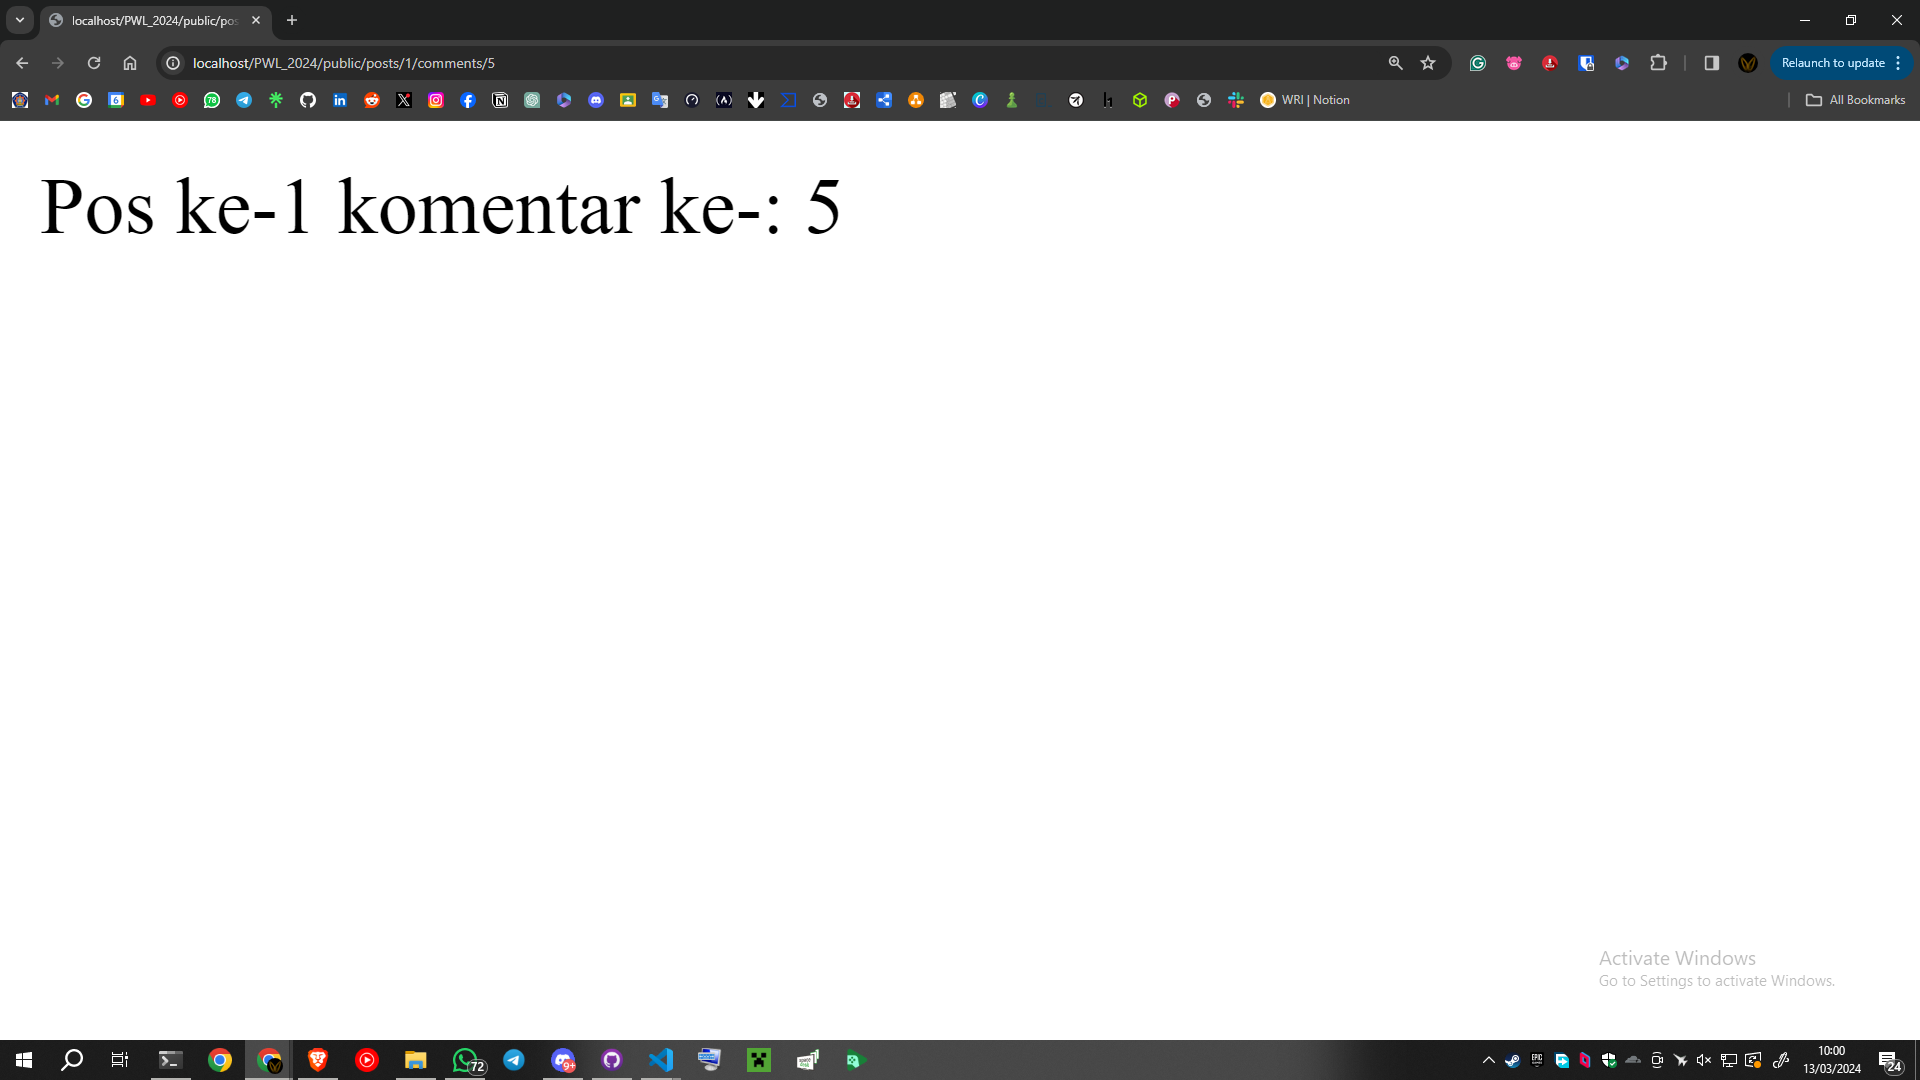
\includegraphics[width=.9\textwidth]{images/figures/route parameters e.png} \\ The text becomes 'Pos ke-1 komentar ke-: 5'
    \item - \\ \includegraphics[width=.9\textwidth]{images/figures/route parameters f.png}
    \begin{minted}[autogobble,breaklines,linenos]{php}
        <?php

        use Illuminate\Support\Facades\Route;
        
        /*
        |--------------------------------------------------------------------------
        | Web Routes
        |--------------------------------------------------------------------------
        |
        | Here is where you can register web routes for your application. These
        | routes are loaded by the RouteServiceProvider and all of them will
        | be assigned to the "web" middleware group. Make something great!
        |
        */
        
        Route::get('/', function () {
            // return view('welcome');
            return 'Welcome';
        });
        
        Route::get('/hello', function () {
            return 'Hello World';
        });
        
        Route::get('/world', function () {
            return 'World';
        }); 
        
        Route::get('/about', function () {
            return '2241720145 - Muhammad Baihaqi Aulia Asyari';
        }); 
        
        Route::get('/user/{name}', function ($name) {
            return 'My name is ' . $name;
        }); 
        
        Route::get('/posts/{post}/comments/{comment}', function ($postId, $commentId) {
            return 'Pos ke-' . $postId . ' komentar ke-: ' . $commentId;
        });
        
        Route::get('/articles/{id}', function ($id) {
            return 'Article Page with ID ' . $id;
        });        
    \end{minted}
\end{enumerate}

\subsection{Optional Parameters}
\begin{enumerate}[label=\alph*.]
    \item -
    \begin{minted}[autogobble,breaklines,linenos]{php}
        <?php

        use Illuminate\Support\Facades\Route;
        
        /*
        |--------------------------------------------------------------------------
        | Web Routes
        |--------------------------------------------------------------------------
        |
        | Here is where you can register web routes for your application. These
        | routes are loaded by the RouteServiceProvider and all of them will
        | be assigned to the "web" middleware group. Make something great!
        |
        */
        
        Route::get('/', function () {
            // return view('welcome');
            return 'Welcome';
        });
        
        Route::get('/hello', function () {
            return 'Hello World';
        });
        
        Route::get('/world', function () {
            return 'World';
        }); 
        
        Route::get('/about', function () {
            return '2241720145 - Muhammad Baihaqi Aulia Asyari';
        }); 
        
        Route::get('/user/{name?}', function ($name=null) {
            return 'My name is ' . $name;
        }); 
        
        Route::get('/posts/{post}/comments/{comment}', function ($postId, $commentId) {
            return 'Pos ke-' . $postId . ' komentar ke-: ' . $commentId;
        });
        
        Route::get('/articles/{id}', function ($id) {
            return 'Article Page with ID ' . $id;
        });      
    \end{minted}
    \item - \\ 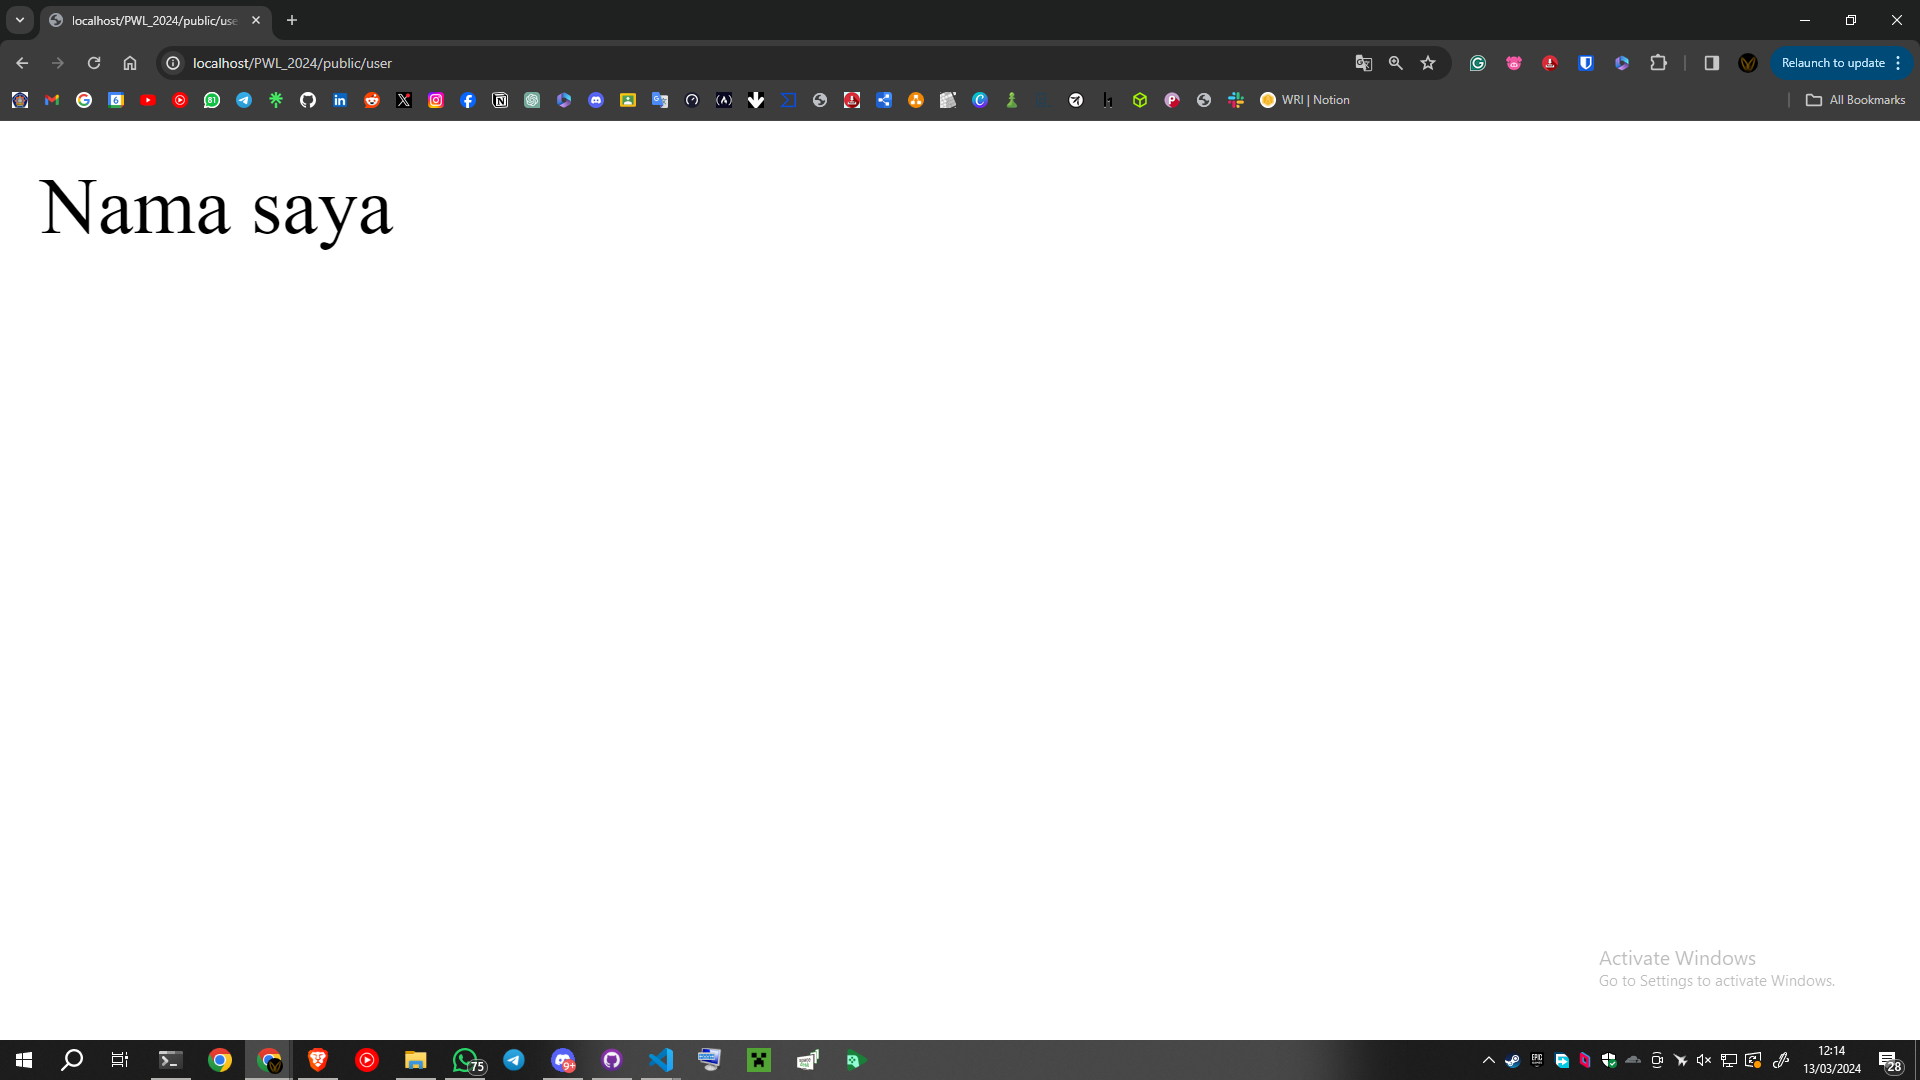
\includegraphics[width=.9\textwidth]{images/figures/optional parameters b.png} \\ now the 404 doesn't appear anymore and the text has becomes 'My name is'
    \item - \\ \includegraphics[width=.9\textwidth]{images/figures/optional parameters c.png} \\ the text can still display the parameter which makes the text 'My name is yourname'
    \item -
    \begin{minted}[autogobble,breaklines,linenos]{php}
        <?php

        use Illuminate\Support\Facades\Route;
        
        /*
        |--------------------------------------------------------------------------
        | Web Routes
        |--------------------------------------------------------------------------
        |
        | Here is where you can register web routes for your application. These
        | routes are loaded by the RouteServiceProvider and all of them will
        | be assigned to the "web" middleware group. Make something great!
        |
        */
        
        Route::get('/', function () {
            // return view('welcome');
            return 'Welcome';
        });
        
        Route::get('/hello', function () {
            return 'Hello World';
        });
        
        Route::get('/world', function () {
            return 'World';
        }); 
        
        Route::get('/about', function () {
            return '2241720145 - Muhammad Baihaqi Aulia Asyari';
        }); 
        
        Route::get('/user/{name?}', function ($name='John') {
            return 'Nama saya ' . $name;
        }); 
        
        Route::get('/posts/{post}/comments/{comment}', function ($postId, $commentId) {
            return 'Pos ke-' . $postId . ' komentar ke-: ' . $commentId;
        });
        
        Route::get('/articles/{id}', function ($id) {
            return 'Article Page with ID ' . $id;
        });        
    \end{minted}
    \item now the default name is John and somehow the language change from english to indonesian
\end{enumerate}

\section{Controller}
\subsection{Creating Controller}

\begin{enumerate}[label=\alph*.]
    \item -
    \begin{minted}[autogobble,breaklines,linenos]{text}
        PS C:\laragon\www\PWL_2024> php artisan make:controller WelcomeController

        INFO  Controller [C:\laragon\www\PWL_2024\app\Http\Controllers\WelcomeController.php] created successfully.
    \end{minted}
    \item -
    \begin{minted}[autogobble,breaklines,linenos]{php}
        <?php

        namespace App\Http\Controllers;
        
        use Illuminate\Http\Request;
        
        class WelcomeController extends Controller
        {
            //
        }
        
    \end{minted}

    \newpage
    
    \item -
    \begin{minted}[autogobble,breaklines,linenos]{php}
        <?php

        namespace App\Http\Controllers;
        
        use Illuminate\Http\Request;
        
        class WelcomeController extends Controller
        {
            public function hello() {
                return 'Hello World';
            }
        }

    \end{minted}
    \item -
    \begin{minted}[autogobble,breaklines,linenos]{php}
        Route::get('/hello', [WelcomeController::class, 'hello']);
    \end{minted}
    \item - \\ 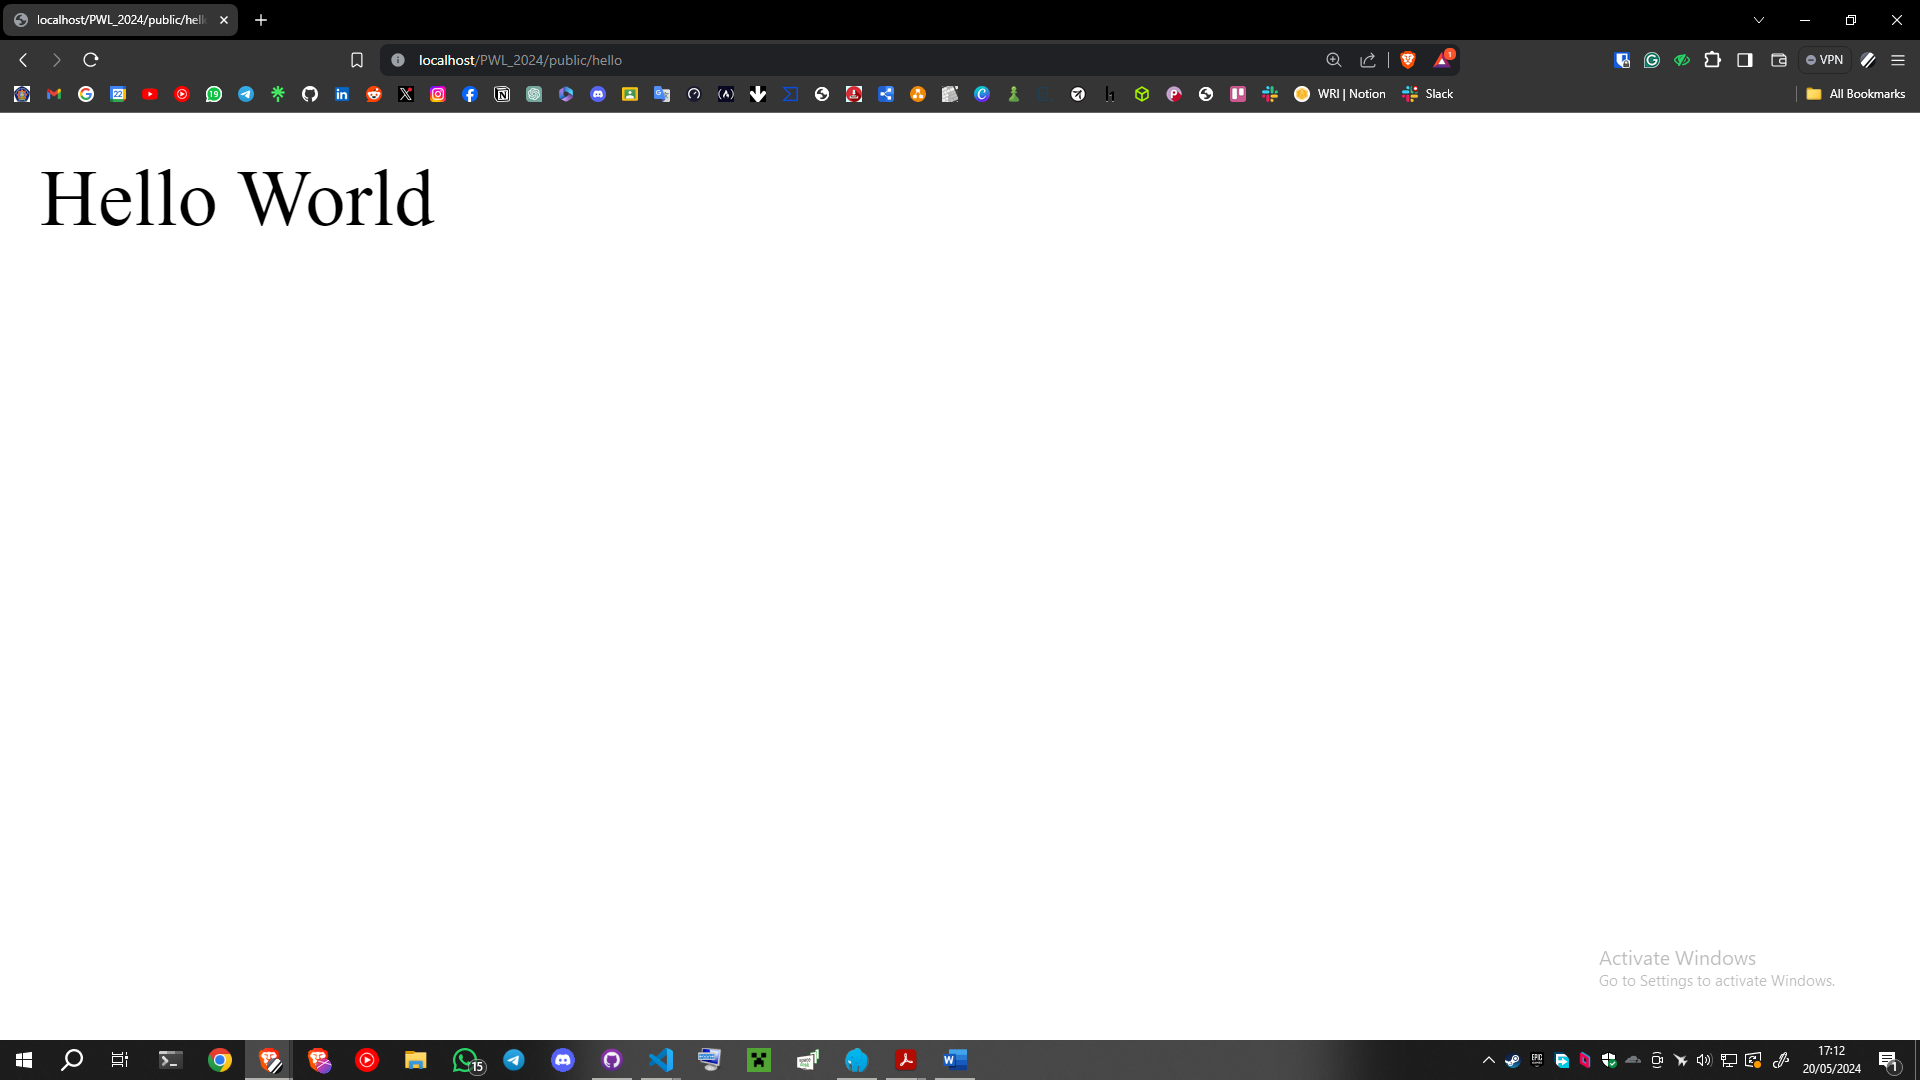
\includegraphics[width=.9\textwidth]{images/figures/creating a controller e.png} \\ it display 'Hello World' text from the controller function

    \newpage

    \item -
    \begin{minted}[autogobble,breaklines,linenos]{php}
        Route::get('/', [PageController::class, 'index']);

        Route::get('/about', [PageController::class, 'about']);

        Route::get('/articles/{id}', [PageController::class, 'articles']);

    \end{minted}

    \begin{minted}[autogobble,breaklines,linenos]{php}
        <?php

        namespace App\Http\Controllers;
        
        use Illuminate\Http\Request;
        
        class PageController extends Controller
        {
            public function index() {
                return 'Welcome';
            }
        
            public function about() {
                return "2241720145 - Muhammad Baihaqi Aulia Asy'ari";
            }
        
            public function articles($id) {
                return 'Article Page with ID ' . $id;
            }
        }

    \end{minted}

    \newpage

    \item -
    \begin{minted}[autogobble,breaklines,linenos]{php}
        <?php

        namespace App\Http\Controllers;
        
        use Illuminate\Http\Request;
        
        class HomeController extends Controller
        {
            public function index() {
                return 'Welcome';
            }
        }
        
    \end{minted}
    \begin{minted}[autogobble,breaklines,linenos]{php}
        <?php

        namespace App\Http\Controllers;
        
        use Illuminate\Http\Request;
        
        class AboutController extends Controller
        {
            public function about() {
                return "2241720145 - Muhammad Baihaqi Aulia Asy'ari";
            }
        }
        
    \end{minted}
    \begin{minted}[autogobble,breaklines,linenos]{php}
        <?php

        namespace App\Http\Controllers;
        
        use Illuminate\Http\Request;
        
        class ArticleController extends Controller
        {
            public function articles($id) {
                return 'Article Page with ID ' . $id;
            }
        }
        
    \end{minted}
    \begin{minted}[autogobble,breaklines,linenos]{php}
        Route::get('/', [HomeController::class, 'index']);

        Route::get('/about', [AboutController::class, 'about']); 

        Route::get('/articles/{id}', [ArticleController::class, 'articles']);

    \end{minted}
\end{enumerate}

\subsection{Resource Controller}
\begin{enumerate}[label=\alph*.]
    \item -
    \begin{minted}[autogobble,breaklines,linenos]{text}
        PS C:\laragon\www\PWL_2024> php artisan make:controller PhotoController --resource

        INFO  Controller [C:\laragon\www\PWL_2024\app\Http\Controllers\PhotoController.php] created successfully. 
    \end{minted}

    \item -
    \begin{minted}[autogobble,breaklines,linenos]{php}
        <?php
        use App\Http\Controllers\PhotoController;
        
        Route::resource('photos', PhotoController::class);
    \end{minted}
    \item -
    \begin{minted}[autogobble,breaklines,linenos]{text}
        PS C:\laragon\www\PWL_2024> php artisan route:list

        GET|HEAD        / ...... ...... ...... ...... ...... ...... ...... ...... .... ...... ...... ...... ...... ...... ...... ...... ...... ...... ...... ..... ......  HomeController@index
        POST            _ignition/execute-solution ...... ...... ...... ...... ...... ...... ..... ignition.executeSolution > Spatie\LaravelIgnition > ExecuteSolutionController  
        GET|HEAD        _ignition/health-check ...... ...... ...... ...... ...... ...... ...... ...... ..... ignition.healthCheck > Spatie\LaravelIgnition > HealthCheckController  
        POST            _ignition/update-config ...... ...... ...... ...... ...... ...... ...... ...... .. ignition.updateConfig > Spatie\LaravelIgnition > UpdateConfigController  
        GET|HEAD        about ...... ...... ...... ...... ...... ...... ...... ...... ...... ......  ...... ...... ...... ...... ...... ...... ...... ...... ...... .... AboutController@about  
        GET|HEAD        articles/{id} ...... ...... ...... ...... ...... ...... ...... ...... ...... ...... . ...... ...... ...... ...... ...... ...... ...... .. ArticleController@articles  
        GET|HEAD        hello ...... ...... ...... ...... ...... ...... ...... ...... ...... ......  ...... ...... ...... ...... ...... ...... ...... ...... ...... .. WelcomeController@hello  
        GET|HEAD        photos ...... ...... ...... ...... ...... ...... ...... ...... ...... ..... ...... ...... ...... ...... ...... ...... ...... . photos.index > PhotoController@index  
        POST            photos ...... ...... ...... ...... ...... ...... ...... ...... ...... ..... ...... ...... ...... ...... ...... ...... ...... . photos.store > PhotoController@store  
        GET|HEAD        photos/create ...... ...... ...... ...... ...... ...... ...... ...... ...... ..... ...... ...... ...... ...... ...... .... photos.create > PhotoController@create  
        GET|HEAD        photos/{photo} ...... ...... ...... ...... ...... ...... ...... ...... ...... .... ...... ...... ...... ...... ...... ...... .. photos.show > PhotoController@show  
        PUT|PATCH       photos/{photo} ...... ...... ...... ...... ...... ...... ...... ...... ...... .... ...... ...... ...... ...... ...... .... photos.update > PhotoController@update  
        DELETE          photos/{photo} ...... ...... ...... ...... ...... ...... ...... ...... ...... .... ...... ...... ...... ...... ...... .. photos.destroy > PhotoController@destroy  
        GET|HEAD        photos/{photo}/edit ...... ...... ...... ...... ...... ...... ...... ...... ...... ...... . ...... ...... ...... ...... ......  photos.edit > PhotoController@edit  
        GET|HEAD        posts/{post}/comments/{comment} ...... ...... ...... ...... ...... ...... ...... ...... ...... .. ...... ...... ...... ...... ...... ...... ...... ...... ...... ....  
        GET|HEAD        sanctum/csrf-cookie ...... ...... ...... ...... ...... ...... ...... ...... ......  ......  sanctum.csrf-cookie > Laravel\Sanctum > CsrfCookieController@show  
        GET|HEAD        user/{name?} ...... ...... ...... ...... ...... ...... ...... ...... ...... .... ...... ...... ...... ...... ...... ...... ...... ...... ...... ...... ..... ...... ....  
        GET|HEAD        world ...... ...... ...... ...... ...... ...... ...... ...... ...... ......  ...... ...... ...... ...... ...... ...... ...... ...... ...... ...... ..... ...... ...... ...
        Showing [19] routes
    \end{minted}
    \item -
    \begin{minted}[autogobble,breaklines,linenos]{php}
        <?php

        use App\Http\Controllers\AboutController;
        use App\Http\Controllers\ArticleController;
        use App\Http\Controllers\HomeController;
        use App\Http\Controllers\PageController;
        use App\Http\Controllers\PhotoController;
        use App\Http\Controllers\WelcomeController;
        use Illuminate\Support\Facades\Route;
        
        /*
        |--------------------------------------------------------------------------
        | Web Routes
        |--------------------------------------------------------------------------
        |
        | Here is where you can register web routes for your application. These
        | routes are loaded by the RouteServiceProvider and all of them will
        | be assigned to the "web" middleware group. Make something great!
        |
        */
        
        Route::get('/', [HomeController::class, 'index']);
        
        Route::get('/hello', [WelcomeController::class, 'hello']);
        
        Route::get('/world', function () {
            return 'World';
        }); 
        
        Route::get('/about', [AboutController::class, 'about']); 
        
        Route::get('/user/{name?}', function ($name='John') {
            return 'Nama saya ' . $name;
        }); 
        
        Route::get('/posts/{post}/comments/{comment}', function ($postId, $commentId) {
            return 'Pos ke-' . $postId . ' komentar ke-: ' . $commentId;
        });
        
        Route::get('/articles/{id}', [ArticleController::class, 'articles']);
        
        Route::resource('photos', PhotoController::class)->only([
            'index', 'show'
        ]);
        
        Route::resource('photos', PhotoController::class)->except([
            'create', 'store', 'update', 'destroy'
        ]);
    \end{minted}
\end{enumerate}

\newpage

\section{View}
\subsection{Creating View}
\begin{enumerate}[label=\alph*.]
    \item -
    \begin{minted}[autogobble,breaklines,linenos]{php}
        {{-- View pada resources/views/hello.blade.php --}}
        <html>
            <body>
                <h1>Hello, {{ $name }}</h1>
            </body>
        </html>
    \end{minted}
    \item -
    \begin{minted}[autogobble,breaklines,linenos]{php}
        Route::get('/greeting', function () {
            return view('hello', ['name' => 'Baihaqi']);
        });
    \end{minted}
    \item - \\ \includegraphics[width=.9\textwidth]{images/figures/creating view c.png}
\end{enumerate}
\newpage
\subsection{View in Directory}
\begin{enumerate}[label=\alph*.]
    \item -
    \item -
    \item -
    \begin{minted}[autogobble,breaklines,linenos]{php}
        Route::get('/greeting', function () {
            return view('blog.hello', ['name' => 'Baihaqi']);
        });
    \end{minted}
    \item - \\ \includegraphics[width=.9\textwidth]{images/figures/view in directory d.png} \\ nothing has change from the previous change except in the background the view now routes to hello inside the blog directory
\end{enumerate}
\newpage
\subsection{Display View from Controller}
\begin{enumerate}[label=\alph*.]
    \item -
    \begin{minted}[autogobble,breaklines,linenos]{php}
        <?php

        namespace App\Http\Controllers;
        
        use Illuminate\Http\Request;
        
        class WelcomeController extends Controller
        {
            public function hello() {
                return 'Hello World';
            }
        
            public function greeting() {
                return view('blog.hello', ['name' => 'Baihaqi']);
            }
        }
    \end{minted}
    \item -
    \begin{minted}[autogobble,breaklines,linenos]{php}
        Route::get('/greeting', [WelcomeController::class, 'greeting']);
    \end{minted}
    \item - \\ 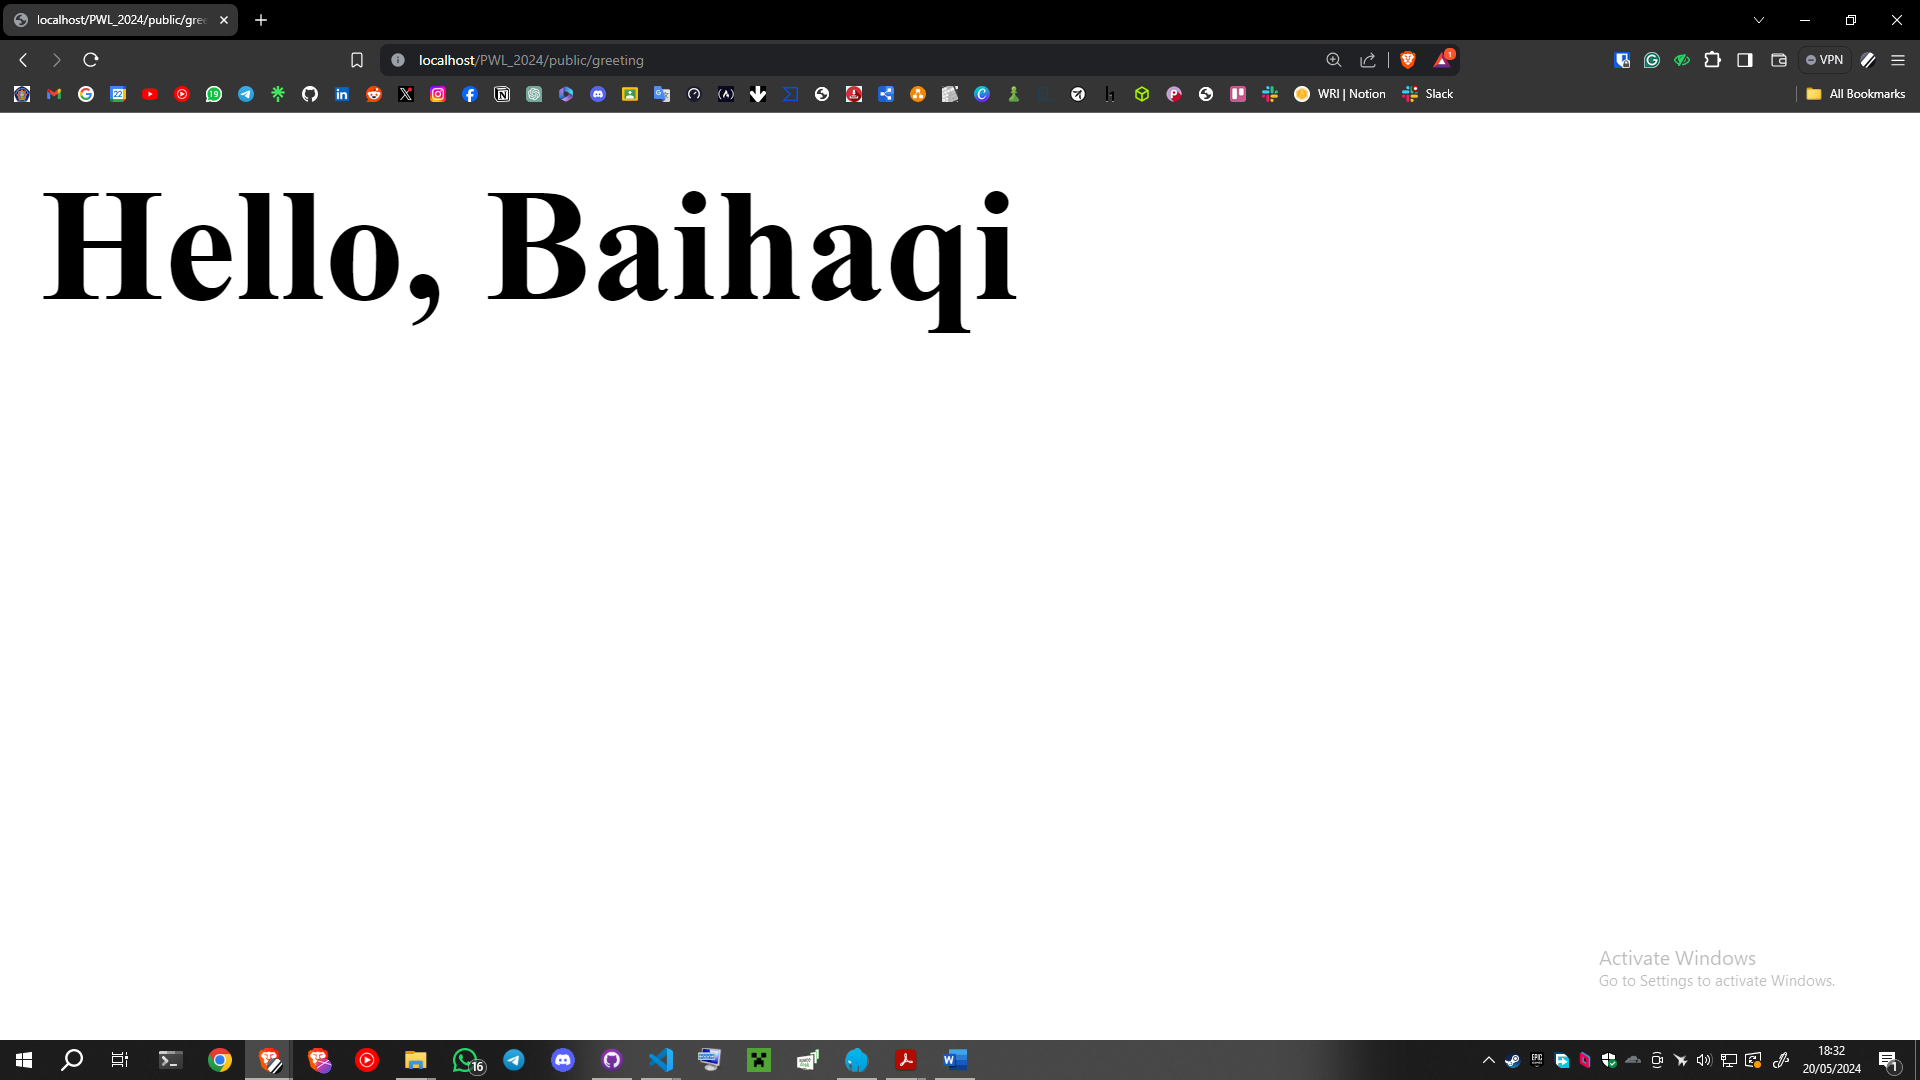
\includegraphics[width=.9\textwidth]{images/figures/Displaying View from Controller c.png}
\end{enumerate}
\subsection{Forward Data to View}
\begin{enumerate}[label=\alph*.]
    \item -
    \begin{minted}[autogobble,breaklines,linenos]{php}
        <?php

        namespace App\Http\Controllers;
        
        use Illuminate\Http\Request;
        
        class WelcomeController extends Controller
        {
            public function hello() {
                return 'Hello World';
            }
        
            public function greeting() {
                return view('blog.hello')
                    ->with('name','Baihaqi')
                    ->with('occupation','Astronaut');
            }
        }
        
    \end{minted}
    \newpage
    \item -
    \begin{minted}[autogobble,breaklines,linenos]{php}
    <html>
        <body>
            <h1>Hello, {{ $name }}</h1>
            <h1>You are {{ $occupation }}</h1>
        </body>
    </html>
    \end{minted}
    \item - \\ 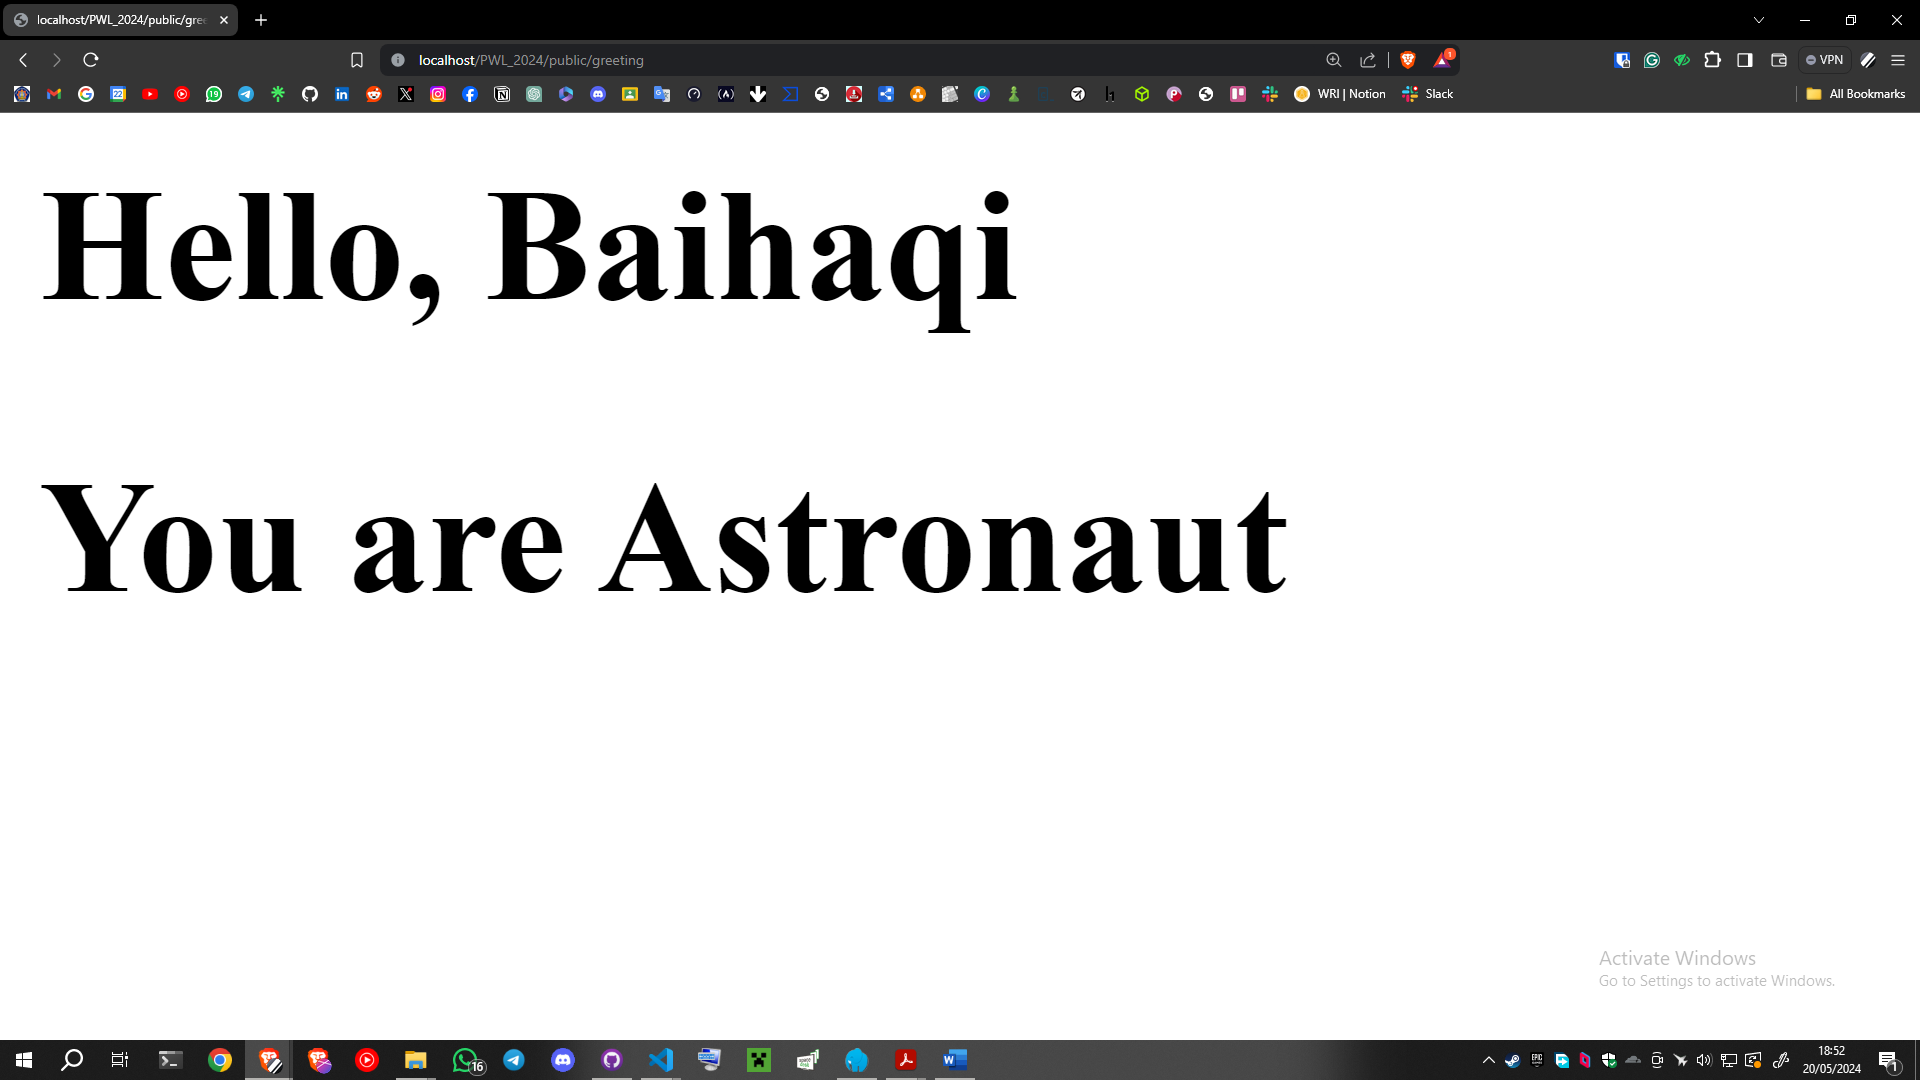
\includegraphics[width=.9\textwidth]{images/figures/forward data to view c.png} \\ now the page display the occupation set in the controller with the with function
\end{enumerate}

\url{https://github.com/G4CENeiz/PWL_2024}

\end{document}